\documentclass[a4paper]{article}
\usepackage{cmap}
\usepackage[utf8]{inputenc}
\usepackage[T2A]{fontenc}
\usepackage[english,russian]{babel} 
\usepackage[left=15mm, top=15mm, right=15mm, bottom=42mm, nohead, nofoot]{geometry}
\usepackage{blindtext}  % рыба-текст
\usepackage{graphicx}  % изобржаения
\usepackage{float} % плавающие объекты
\usepackage{wrapfig}  % изобржаения
\usepackage{tikz} % графика
\usepackage{xcolor} % определение цветов
\usepackage{nicefrac} % красивые дроби
\usepackage{cancel} % сокращение
\usepackage{amsmath,amsfonts,amssymb} % математический пакет
\usepackage{hyperref}  % гиперссылки
\usepackage{fancybox,fancyhdr} % хедер и футер
\usepackage{listings} % код
\usepackage{accsupp}
\usepackage{caption}

\captionsetup[figure]{name=Рисунок}
\pagestyle{fancy}
\fancyhf{}
\fancyhead[L]{Лабораторная работа №5}
\fancyhead[R]{\textit{Типовые динамические звенья}}
\fancyfoot[C]{\thepage}
\headsep=8mm
\footskip=20mm

\definecolor{urlcolor}{HTML}{3454D1}
\definecolor{linkcolor}{HTML}{3454D1}
\hypersetup{pdfstartview=FitH, linkcolor=linkcolor, urlcolor=urlcolor, colorlinks=true}

\definecolor{strings}{rgb}{0,0.6,0}
\definecolor{comments}{rgb}{0,0.3,0}
\definecolor{numbers}{rgb}{0.5,0.5,0.5}
\definecolor{keywords}{rgb}{0.09,0.61,0.95}
\definecolor{background}{rgb}{0.97,0.97,0.97}
\newcommand{\noncopynumber}[1]{%
    \BeginAccSupp{method=escape,ActualText={}}%
    #1%
    \EndAccSupp{}%
}
\lstdefinestyle{codestyle}{
    backgroundcolor=\color{background},
    commentstyle=\color{comments},
    keywordstyle=\color{keywords},
    stringstyle=\color{strings},
    numberstyle=\tiny\color{numbers}\noncopynumber,
    basicstyle=\ttfamily\footnotesize,
    breakatwhitespace=false,
    breaklines=true,
    captionpos=b,
    inputencoding=utf8,
    keepspaces=true,
    numbers=left,
    numbersep=5pt,
    showspaces=false,
    showstringspaces=false,
    showtabs=false,
    tabsize=2,
    extendedchars=true,
    literate=
    {а}{{\cyra}}1
    {б}{{\cyrb}}1
    {в}{{\cyrv}}1
    {г}{{\cyrg}}1
    {д}{{\cyrd}}1
    {е}{{\cyre}}1
    {ж}{{\cyrzh}}1
    {з}{{\cyrz}}1
    {и}{{\cyri}}1
    {й}{{\cyrishrt}}1
    {к}{{\cyrk}}1
    {л}{{\cyrl}}1
    {м}{{\cyrm}}1
    {н}{{\cyrn}}1
    {о}{{\cyro}}1
    {п}{{\cyrp}}1
    {р}{{\cyrr}}1
    {с}{{\cyrs}}1
    {т}{{\cyrt}}1
    {у}{{\cyru}}1
    {ф}{{\cyrf}}1
    {х}{{\cyrh}}1
    {ц}{{\cyrc}}1
    {ч}{{\cyrch}}1
    {ш}{{\cyrsh}}1
    {щ}{{\cyrshch}}1
    {ъ}{{\cyrhrdsn}}1
    {ы}{{\cyrery}}1
    {ь}{{\cyrsftsn}}1
    {э}{{\cyrerev}}1
    {ю}{{\cyryu}}1
    {я}{{\cyrya}}1
    {А}{{\CYRA}}1
    {Б}{{\CYRB}}1
    {В}{{\CYRV}}1
    {Г}{{\CYRG}}1
    {Д}{{\CYR96}}1
    {Е}{{\CYRE}}1
    {Ж}{{\CYRZH}}1
    {З}{{\CYRZ}}1
    {И}{{\CYRI}}1
    {Й}{{\CYRISHRT}}1
    {К}{{\CYRK}}1
    {Л}{{\CYRL}}1
    {М}{{\CYRM}}1
    {Н}{{\CYRN}}1
    {О}{{\CYRO}}1
    {П}{{\CYRP}}1
    {Р}{{\CYRR}}1
    {С}{{\CYRS}}1
    {Т}{{\CYRT}}1
    {У}{{\CYRU}}1
    {Ф}{{\CYRF}}1
    {Х}{{\CYRH}}1
    {Ц}{{\CYRC}}1
    {Ч}{{\CYRCH}}1
    {Ш}{{\CYRSH}}1
    {Щ}{{\CYRSHCH}}1
    {Ъ}{{\CYRHRDSN}}1
    {Ы}{{\CYRERY}}1
    {Ь}{{\CYRSFTSN}}1
    {Э}{{\CYREREV}}1
    {Ю}{{\CYRYU}}1
    {Я}{{\CYRYA}}1
}

\lstset{style=codestyle}

\addto\captionsrussian{
  \renewcommand{\contentsname}
    {\centering Содержание}
}


\newlength{\tempheight}
% \newcommand{\Let}{
% \mathbin{\text{\settoheight{\tempheight}{\mathstrut}\raisebox{0.4\pgflinewidth}{
% \tikz[baseline=0.5ex,line cap=round,line join=round] \draw (0,0) --++ (0.3em,0) --++ (0,2.3ex) --++ (-0.3em,0);
% }}}}
\newcommand*\squared[1]{\tikz[baseline=(char.base)]{
            \node[shape=rectangle,draw,inner sep=4pt] (char) {#1};}}
\newcommand*\msquared[1]{\tikz[baseline=(char.base)]{
            \node[shape=rectangle,draw,inner sep=4pt] (char) {$\displaystyle #1$};}}
\newcommand{\at}{\biggr\rvert}
\newcommand{\shiftright}[3]{\makebox[#2][r]{\makebox[#1][l]{#3}}}
\newcommand{\e}{\;\text{e}}
\let\oldint\int
\def\int{\oldint\limits}
\DeclareRobustCommand{\divby}{%
  \mathrel{\vbox{\baselineskip.65ex\lineskiplimit0pt\hbox{.}\hbox{.}\hbox{.}}}%
}

\newcommand\NB{\textbf{N\kern-0.32em\textcolor{red}{B}}}

\begin{document}

\begin{titlepage}
    \begin{center}
        Федеральное государственное автономное образовательное \\ учреждение высшего образования \\[6pt]
        САНКТ-ПЕТЕРБУРГСКИЙ НАЦИОНАЛЬНЫЙ \\ ИССЛЕДОВАТЕЛЬСКИЙ УНИВЕРСИТЕТ ИТМО \\[16pt]
        Факультет систем управления и робототехники \\[26em]
        Лабораторная работа №5\\[0.5em]
        \textbf{ТИПОВЫЕ ДИНАМИЧЕСКИЕ ЗВЕНЬЯ}
    \end{center}\,\\[10em]
    \begin{flushright}
        Студент: Заводин Е.Ю.\\
        Лин САУ R23 бак 1.1.1 \\[0.5em]
        Преподаватели: Перегудин А.А.\\
        Пашенко А.В.
    \end{flushright}\,\\[6em]
    \begin{center}
        {\small Санкт-Петербург \\ 2025}
    \end{center}
\end{titlepage}
\setcounter{page}{2}
\tableofcontents\newpage

\section{Задача исследования типовых динамических звеньев}\

В работе исследуются реальные объекты --- находятся их передаточные функции, сопоставляются с типовыми звеньями, временные и частотные характеристики объектов моделируются и сравниваются с конкретными теоретическими для найденных типовых звеньев.

Временными характеристиками системы являются её весовая и переходная функции, то есть ответ системы соответственно на дельта-функцию в качестве входного воздействия и ответ на единичный скачок, тогда весовая функция может быть определена по следующей формуле:

\[
w(t) = \mathcal{L}^{-1}\left\{W(s)\cdot\mathcal{L}\{\delta(t)\}\right\} = \mathcal{L}^{-1}\left\{W(s)\cdot1\right\} = \mathcal{L}^{-1}\left\{W(s)\right\},
\]
где $W(s)$ --- передаточная функция системы.

Тогда переходная функция, являющаяся ответом системы на единичный скачок, определяется следующей формулой:

\[
y_{s.r.} = \mathcal{L}^{-1}\left\{W(s)\cdot\mathcal{L}\{1\}\right\} = \mathcal{L}^{-1}\left\{W(s)\cdot\frac{1}{s}\right\} = \mathcal{L}^{-1}\left\{\frac{W(s)}{s}\right\}.
\]

В качестве частотных характеристик рассматриваются АЧХ, ФЧХ, ЛАЧХ, ЛФЧХ. Формулы для расчета АЧХ $A(\omega)$ и ФЧХ $\varphi(\omega)$ следующие:

\[
A(\omega) = \sqrt{P(\omega)^2 + Q(\omega)^2}, \,\,\,\varphi(\omega) = \text{atan2}\left(Q(\omega), P(\omega)\right),
\]
где $P(\omega), Q(\omega)$ --- соответственно действительная и мнимая части частотной передаточной функции $W(\omega) = P(\omega) + jQ(\omega)$.

Выражение для ЛФЧХ ничем не будет отличаться от такового для ФЧХ, но ЛАЧХ отлична от АЧХ:

\[
L(\omega) = 20\lg{\left(\frac{A(\omega)}{A_\text{б}}\right)}, A_\text{б} = 1.
\]

\subsection{ДПТ}\

Рассмотрим ДПТ независимого возбуждения, задаваемый формулами

\[
J\dot{\omega} = M, M = k_mI, I = \frac{U + \varepsilon_i}{R}, \varepsilon_i = -k_e\omega. 
\]\

Считая $U$ входом, $\omega$ --- выходом, сведу формулы к одному линейному дифференциальному уравнению:

\[
J\dot{\omega} = k_m \frac{U-k_e\omega}{R} = \frac{Uk_e}{R} - \frac{k_mk_e\omega}{R}
\]

\[
J\dot{\omega} + \frac{k_mk_e \omega}{R} = \frac{k_m}{R} U
\]

\[
\frac{JR}{k_m}\dot{\omega} + k_e\omega = U
\]

\[
\frac{\omega}{U} = W(s) = \frac{1}{\frac{JR}{k_m}s + k_e} = \frac{1}{k_e} \frac{1}{\frac{JR}{k_ek_m}s + 1}
\]

\[
W(s) = \frac{K}{Ts+1}, T = \frac{JR}{k_ek_m}, K = \frac{1}{k_e}
\]\ 

Получил передаточную функцию в стандартизированном виде, соответствующую реальному усилительному звену. 

\subsubsection{Частотные характеристики}\

Выделю действительную и мнимую части полученной передаточной функции:

\[
W(s) = \frac{K}{Ts+1} \Rightarrow W(j\omega) = \frac{K}{T(j\omega)+1}
\]

\[
W(j\omega) = \frac{K}{1 + j T \omega} \cdot \frac{1 - j T \omega}{1 - j T \omega}
= \frac{K(1 - j T \omega)}{1 + (T \omega)^2}
= \frac{K}{1 + (T \omega)^2} + j \frac{-K T \omega}{1 + (T \omega)^2}
\]\

Пусть $P(\omega) = \frac{K}{1 + (T \omega)^2}$, $Q(\omega) = \frac{-K T \omega}{1 + (T \omega)^2}$. Рассчитаю АЧХ такой передаточной функции:

\[
A(\omega) = \sqrt{P(\omega)^2 + Q(\omega)^2}
= \sqrt{ \frac{K^2 + (K T \omega)^2}{\big(1 + (T \omega)^2\big)^2} }
= \frac{K \sqrt{1 + (T \omega)^2}}{1 + (T \omega)^2}
= \frac{K}{\sqrt{1 + (T \omega)^2}}
\]

Тогда ЛАЧХ будет выглядеть так:

\[
L(\omega) = 20 \lg \left( \frac{K}{\sqrt{1 + (T \omega)^2}} \right)
\]

Разложим логарифм:

\[
L(\omega) = 20 \lg(K) - 10 \lg\left(1 + (T \omega)^2\right).
\]

Фазовая частотная характеристика может быть найдена по следующей формуле:

\[
\varphi(\omega) = \text{atan}2(Q(\omega), P(\omega)).
\]\ 

У двигателя постоянного тока активное сопротивление обмоток ротора $R$, момент инерции ротора $J$ и конструктивные постоянные $k_e, k_m$ при реальном моделировании являются положительными, также буду считать, что $\omega$ принимает только неотрицательные значения (в отрицательной области для вещественной функции результат преобразования Лапласа будет симметричен результату в положительной области). Исходя из этого, коэффициент усиления и постоянная времени

\[
T = \frac{JR}{k_ek_m} > 0, K = \frac{1}{k_e} > 0.
\]\ 

Тогда числитель действительной части передаточной функции всегда положителен, как и знаменатель, а значит, $P(\omega) > 0$. Числитель мнимой части передаточной функции же всегда отрицателен, а знаменатель всегда положителен, следовательно, $Q(\omega) < 0$. Исходя из этих соображений, комплексное число $W(j\omega) = P(\omega) +jQ(\omega)$ находится в четвёртом квадранте, а значит, вместо $\text{atan}2{(Q(\omega), P(\omega))}$ можем использовать $\arctan{\left(\frac{Q(\omega)}{P(\omega)}\right)}$:

\[
\arctan{\left(\frac{Q(\omega)}{P(\omega)}\right)} = \arctan{\left(\frac{\frac{-KT\omega}{1+(T\omega)^2}}{\frac{K}{1+(T\omega)^2}}\right)} = 
\arctan{\left(\frac{-KT\omega}{K}\right)} = 
\arctan{-T\omega} = -\arctan{T\omega}
\]

Подставляя значения исходных данных для своего варианта, получаю 

\[
K = \frac{1}{k_e} = \frac{1}{0.3612} \approx 2.7685, T = \frac{JR}{k_ek_m} = \frac{0.0031 \cdot 4.7231}{0.3612 \cdot 0.3612} \approx 0.1122 \Rightarrow W(s) = \frac{2.7685}{0.1122s + 1}
\]

\[
A(\omega) = \frac{K}{\sqrt{1 + (T\omega)^2}} = \frac{2.7685}{\sqrt{1 + (0.1122\omega)^2}}
\]

\[
L(\omega) = 20 \lg \left(\frac{2.7685}{\sqrt{1 + (0.1122\omega)^2}}\right)
\]

\[
\varphi(\omega) = -\text{arctan}(0.1122\omega).
\]

\subsubsection*{Моделирование}\

Полученная передаточная функция была промоделирована, и результаты моделирования были сопоставлены с полученными аналитически:

\begin{figure}[H]
    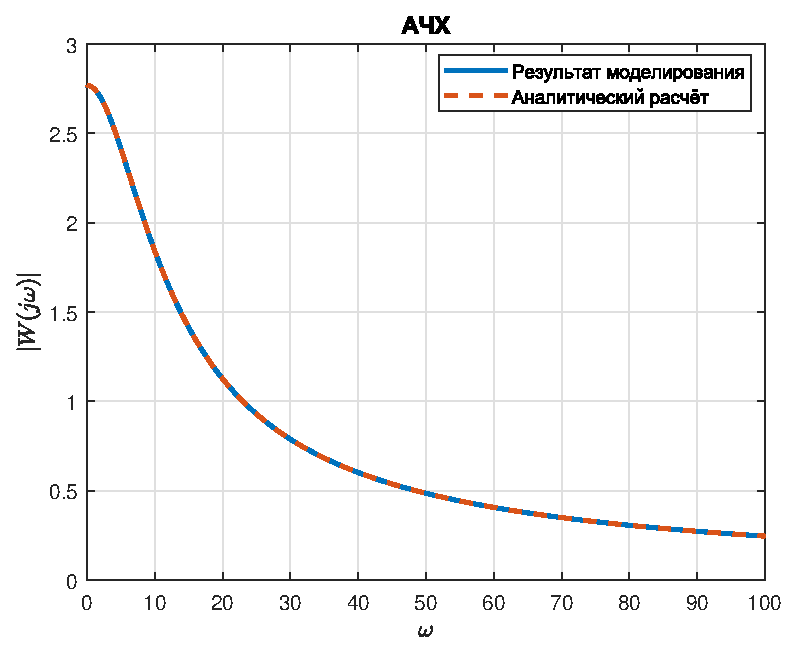
\includegraphics[width=0.65\linewidth]{ex1/achh.eps}
    \centering
    \caption{Сравнение АЧХ промоделированной системы с аналитически рассчитанной АЧХ}
\end{figure}

\begin{figure}[H]
    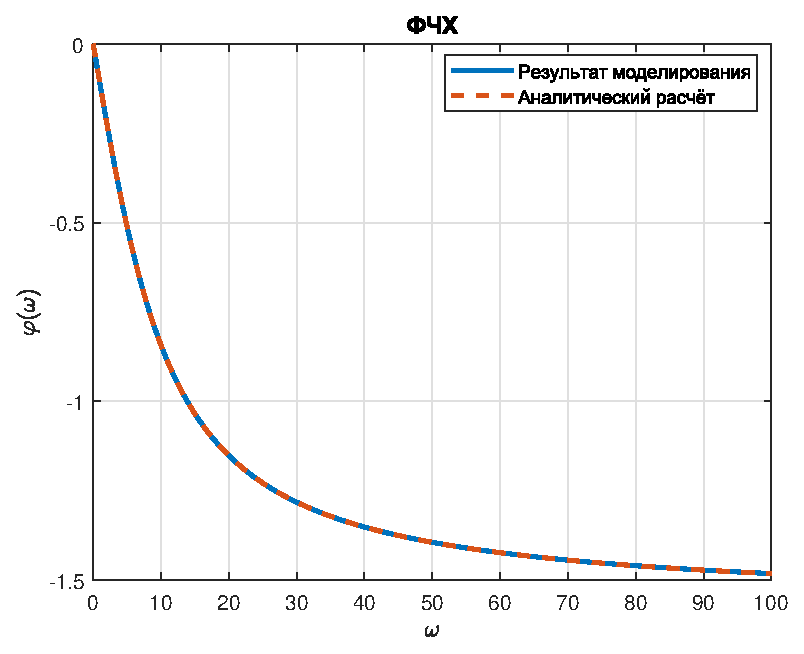
\includegraphics[width=0.65\linewidth]{ex1/fchh.eps}
    \centering
    \caption{Сравнение ФЧХ промоделированной системы с аналитически рассчитанной ФЧХ}
\end{figure}

\begin{figure}[H]
    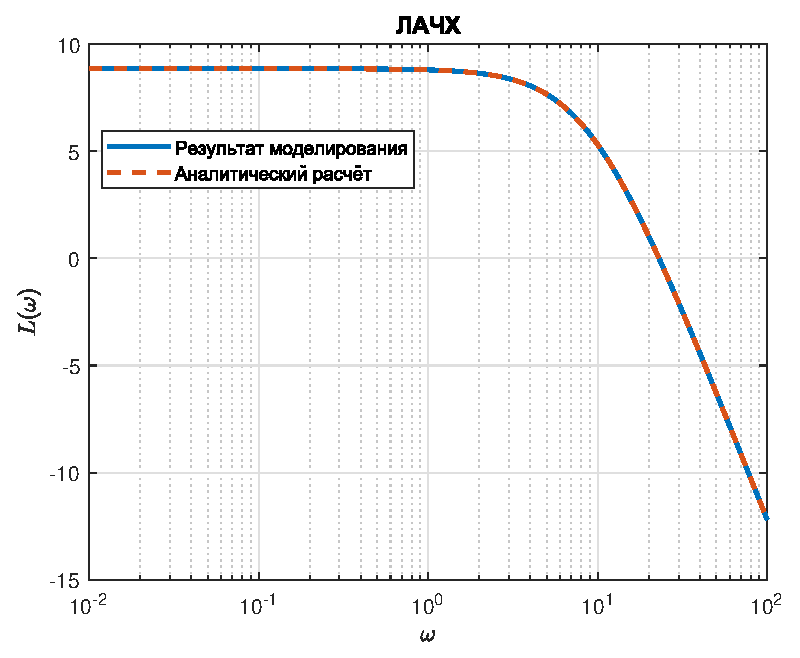
\includegraphics[width=0.65\linewidth]{ex1/lachh.eps}
    \centering
    \caption{Сравнение ЛАЧХ промоделированной системы с аналитически рассчитанной ЛАЧХ}
\end{figure}

\begin{figure}[H]
    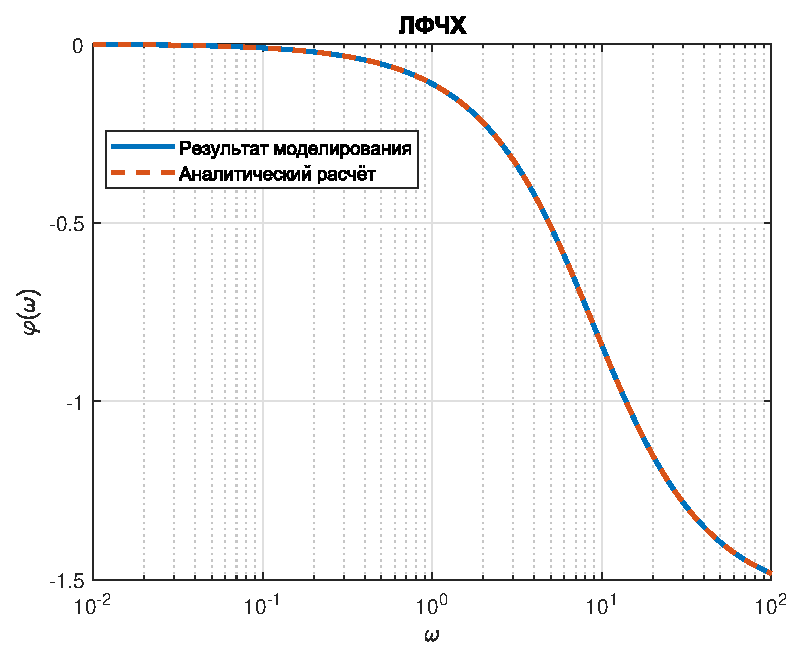
\includegraphics[width=0.65\linewidth]{ex1/lfchh.eps}
    \centering
    \caption{Сравнение ЛФЧХ промоделированной системы с аналитически рассчитанной ЛФЧХ}
\end{figure}

Результаты полученных графических представлений частотных характеристик полностью совпали с теоретическими для рассмотренного реального усилительного звена.

\subsubsection{Временные характеристики}\

Весовая функция объекта:

\[
w(t) = \mathcal{L}^{-1}\{W(s)\} = \mathcal{L}^{-1}\left\{\frac{K}{Ts+1}\right\} = \mathcal{L}^{-1}\left\{\frac{K/T}{s+1/T}\right\} = \frac{K}{T}\mathcal{L}^{-1}\left\{\frac{1}{s+1/T}\right\}
\]

Воспользуемся табличным преобразованием:

\[
\mathcal{L}\{e^{\alpha t}\} = \frac{1}{s-\alpha} \Rightarrow \mathcal{L}^{-1}\left\{\frac{1}{s-\alpha}\right\} = e^{\alpha t}
\]

Тогда, при $\alpha = -\frac{1}{T}$:

\[
w(t) = \frac{K}{T}\mathcal{L}^{-1}\left\{\frac{1}{s+1/T}\right\} = \frac{K}{T} e^{-\frac{1}{T}t}.
\]

Переходная функция:

\[
y_{s.r.}(t) = \mathcal{L}^{-1}{\frac{W(s)}{s}} = \mathcal{L}^{-1}\left\{\frac{K}{s(Ts+1)}\right\} = \mathcal{L}^{-1}\left\{\frac{K/T}{s^2+s/T}\right\} = \frac{K}{T}\mathcal{L}^{-1}\left\{\frac{1}{s^2+s/T}\right\} = \frac{K}{T}\mathcal{L}^{-1}\left\{\frac{1}{s}\frac{1}{s+1/T}\right\}.
\]

По свойству интегрирования:

\[
\frac{K}{T}\mathcal{L}^{-1}\left\{\frac{1}{s}\frac{1}{s+1/T}\right\} = \frac{K}{T}\int_{0^-}^{t}\mathcal{L}^{-1}\left\{\frac{1}{s+1/T}\right\}.
\]

Воспользуемся уже вычисленным при нахождении весовой функции значением:

\[
\frac{K}{T}\int_{0^-}^{t}\mathcal{L}^{-1}\left\{\frac{1}{s+1/T}\right\} = \frac{K}{T}\int_{0^-}^{t}e^{-\frac{1}{T}x}dx.
\]

Рассмотрим неопределенный интеграл $\int e^{-\frac{1}{T}x}dx$:

\[
F(x) = \int e^{-\frac{1}{T}x}dx = -T e^{-\frac{x}{T}}+ C.
\]

Первообразная найдена, можем посчитать определенный интеграл:

\[
y_{s.r}(t) = \frac{K}{T}\int_{0^-}^{t} e^{-\frac{1}{T}x}dx = \frac{K}{T}\left( F(t) - F(0^-)\right) =\frac{K}{T}\left( -T e^{-\frac{t}{T}} + T e^{0} \right)= K(1 - e^{\frac{-t}{T}}).
\]

Подставлю исходные данные для своего варианта в полученные характеристики:

\[
K = 2.7685, T = 0.1122 \Rightarrow w(t) = \frac{K}{T} e^{-\frac{1}{T}t} = \frac{2.7685}{0.1122}e^{-\frac{1}{0.1122}t} = 24.6747e^{-8.9127t}
\]

\[
y_\text{s.r.} = K(1 - e^{\frac{-t}{T}}) = 2.7685(1 - e^{-8.9127t}).
\]

\subsubsection*{Моделирование}\

Снова проведя моделирование, я получил временные характеристики системы, и сопоставил их с полученными аналитически:

\begin{figure}[H]
    \includegraphics[width=0.65\linewidth]{ex1/step.eps}
    \centering
    \caption{Сравнение промоделированной переходной функции с полученной аналитически}
\end{figure}

\begin{figure}[H]
    \includegraphics[width=0.65\linewidth]{ex1/impulse.eps}
    \centering
    \caption{Сравнение промоделированной весовой функции с полученной аналитически}
\end{figure}

Результаты полученных графических представлений временных характеристик полностью совпали с теоретическими для рассмотренного реального усилительного звена.

\subsection{ДПТ 2.0}\

Рассмотрим уравнения для полной модели ДПТ независимого возбуждения: 

\[
J\dot{\omega} = M, M = k_mI, I = \frac{U + \varepsilon}{R}, \varepsilon = \varepsilon_i + \varepsilon_s, \varepsilon_i = -k_e\omega, \varepsilon_s = -L\dot{I}. 
\]\

Считая $U$ входом, $\omega$ --- выходом, сведём формулы к одному линейному дифференциальному уравнению:

\[
J\dot{\omega} = k_m \frac{U-k_e\omega -L\dot{I}}{R} = \left.\frac{k_m}{R}U - \frac{k_mk_e\omega}{R}\omega - \frac{L\dot{I}k_m}{R}\right|\cdot \frac{R}{k_m}
\]

\[
\frac{JR}{k_m}\dot\omega+k_e\omega + L\dot I = U
\]

\[
J\dot\omega = k_mI \Rightarrow I = \frac{J\dot \omega}{k_m}, \dot I = \frac{J\ddot \omega}{k_m}
\]

\[
\frac{JL}{k_m}\ddot\omega +\frac{JR}{k_m}\dot\omega + k_e\omega = U \Leftrightarrow \ddot \omega +\frac{R}{L}\dot \omega +\frac{k_ek_m}{J}\omega = \frac{k_m}{J}U
\]\

Переведу получившееся уравнение в пространство изображений Лаплпаса:

\[
s^2\Omega(s) +\frac{R}{L}s\Omega(s) + \frac{k_e k_m}{J}\Omega(s) = \frac{k_m}{J}U(s)
\]

\[
W(s) = \frac{U(s)}{\Omega(s)} = \frac{\frac{k_m}{J}}{s^2 + \frac{R}{L}s + \frac{k_ek_m}{J}} = \frac{\frac{1}{k_e}}{\frac{J}{k_ek_m}s^2+\frac{RJ}{k_ek_mL}s + 1}
\]\

\[
W(s) = \frac{K}{T^2s^2 + 2T\xi s + 1}, K = \frac{1}{k_e}, T = \sqrt{\frac{J}{k_ek_m}}, \xi = \frac{TR}{2L}
\]\

Получена передаточная функция в стандартизированном виде. Для определения конкретного типа звена объекта найду дискриминант знаменателя передаточной функции объекта, подставив параметры $T, \xi$ в соответствии со своим вариантом:

\[T = \sqrt{\frac{J}{k_ek_m}} = \sqrt{\frac{0.0031}{0.3612\cdot0.3612}} \approx 0.1541,\]

\[
\xi = \frac{TR}{2L} = \frac{0.154\cdot4.7237}{2\cdot1.0567} \approx 0.3445.
\]

Тогда, 

\[
D = (2T\xi)^2 - 4(T^2) = (2\cdot0.1541\cdot0.3445)^2-4\cdot0.1541^2 = (0.0858)^2 - 4\cdot 0.0237 \approx -0.009
\]

Получается что корни знаменателя комплексно-сопряженные, а значит, функция соответствует колебательному звену. Для выделения действительной и мнимой части сперва перейду к частотной передаточной функции:

\[
W(s) = \frac{K}{T^2s^2 + 2T\xi s + 1} \Rightarrow W(j\omega) = \frac{K}{T^2(j\omega)^2 + 2T\xi (j\omega) + 1}
\]

\[
W(j\omega) = \frac{K(T^2(j\omega)^2 + 1 - 2T\xi (j\omega))}{(T^2(j\omega)^2 + 2T\xi (j\omega) + 1)(T^2(j\omega)^2 + 1 - 2T\xi (j\omega))} = \frac{K(-T^2\omega^2 + 1 - 2T\xi (j\omega))}{(-T^2\omega^2 + 1 + j2T\xi \omega)(-T^2\omega^2 + 1 - j2T\xi \omega)} = 
\]

\[
= \frac{K(-T^2\omega^2 + 1 - 2T\xi (j\omega))}{(1-T^2\omega^2)^2+(2T\xi\omega)^2} = \frac{K-KT^2\omega^2}{(1-T^2\omega^2)^2+(2T\xi\omega)^2} +j\frac{-2KT\xi \omega}{(1-T^2\omega^2)^2+(2T\xi\omega)^2}.
\]\

Пусть $P(\omega) = \frac{K-KT^2\omega^2}{(1-T^2\omega^2)^2+(2T\xi\omega)^2}, Q(\omega) = \frac{-2KT\xi \omega}{(1-T^2\omega^2)^2+(2T\xi\omega)^2}.$ 

\subsubsection{Частотные характеристики}\

Рассчитаю амплитудно-частотную характеристику:

\[
A(\omega) = \sqrt{\left(\frac{-2KT\xi \omega}{(1-T^2\omega^2)^2+(2T\xi\omega)^2}\right)^2 + \left(\frac{K-KT^2\omega^2}{(1-T^2\omega^2)^2+(2T\xi\omega)^2}\right)^2} = \sqrt{\frac{4K^2T^2\xi^2\omega^2 + K^2-2K^2T^2\omega^2 + K^2T^4\omega^4}{\left((1-T^2\omega^2)^2+(2T\xi\omega)^2\right)^2}}=
\]

\[=
K\sqrt{\frac{4T^2\xi^2\omega^2-2T^2\omega^2 + T^4\omega^4 + 1}{\left((1-T^2\omega^2)^2+(2T\xi\omega)^2\right)^2}} = K\sqrt{\frac{T^2\omega^2(4\xi^2-2 + T^2\omega^2) + 1}{\left((1-T^2\omega^2)^2+(2T\xi\omega)^2\right)^2}}.
\]\

Тогда ЛАЧХ:

\[
L(\omega) = 20 \lg K \sqrt{\frac{ T^2\omega^2(4\xi^2 - 2 + T^2\omega^2) + 1 }{ \left( (1 - T^2\omega^2)^2 + (2T\xi\omega)^2 \right)^2 }} = 20 \lg K + 20 \cdot \frac{1}{2} \lg \left( \frac{ T^2\omega^2(4\xi^2 - 2 + T^2\omega^2) + 1 }{ \left( (1 - T^2\omega^2)^2 + (2T\xi\omega)^2 \right)^2 } \right)=
\]

\[
= 20 \lg K + 10 \lg \left( T^2\omega^2(4\xi^2 - 2 + T^2\omega^2) + 1 \right) - 10 \lg \left( \left( (1 - T^2\omega^2)^2 + (2T\xi\omega)^2 \right)^2 \right)=
\]

\[
= 20 \lg K + 10 \lg \left( T^2\omega^2(4\xi^2 - 2 + T^2\omega^2) + 1 \right) - 20 \lg \left( (1 - T^2\omega^2)^2 + (2T\xi\omega)^2 \right).
\]

Фазовая частотная характеристика будет определяться следующим образом:

\[
\varphi(\omega) = \text{atan2}(Q(\omega), P(\omega)) = \text{atan2}\left(\frac{-2KT\xi \omega}{(1-T^2\omega^2)^2+(2T\xi\omega)^2}, \frac{K-KT^2\omega^2}{(1-T^2\omega^2)^2+(2T\xi\omega)^2}\right)
\]\

Расположение $W(j\omega) = P(\omega) +jQ(\omega)$ на комплексной плоскости, а значит, и оценка фазовой частотной характеристики, определяется в зависимости от того, положительные ли значения принимают $P(\omega)$ и $Q(\omega)$.\

Знаменатели $P(\omega)$ и $Q(\omega)$ всегда положительны. Тогда знаки вещественной и мнимой части $W(j\omega)$ определяются их числителями --- $Q(\omega) < 0$ (т.к. $K, T, \xi > 0$), знак $P(\omega)$ меняется в зависимости от значения $\omega$.\

Рассмотрим $P(\omega) > 0$:

\[
\frac{1-T^2\omega^2}{\left((1-T^2\omega^2)^2+(2T\xi\omega)^2\right)^2} > 0 \Leftrightarrow 1-T^2\omega^2 > 0 \Leftrightarrow \omega< \frac{1}{T}
\]
Тогда $P(\omega) > 0$ при $\omega >\frac{1}{T}$, $P(\omega) = 0$ при $\omega = \frac{1}{T}$. следовательно:\

При $0 \leq \omega < \frac{1}{T}$ $W(j\omega)$ находится в четвертом квадранте, значит, 
\[
\varphi(\omega) = \text{atan2}(Q(\omega), P(\omega)) = \arctan\left(\frac{Q(\omega)}{P(\omega)}\right) = -\arctan\!\left( \frac{2T\xi\omega}{1 - T^2\omega^2} \right).
\]\

При $\omega = \frac{1}{T}$ $W(j\omega)$ $P(\omega) = Q(\omega) = 0 \Rightarrow \varphi = -\frac{\pi}{2}.$\

При $\omega > \frac{1}{T}$ $W(j\omega)$ в третьем квадранте, а значит, 

\[
\varphi(\omega) = \text{atan2}(Q(\omega), P(\omega)) = \arctan\left(\frac{Q(\omega)}{P(\omega)}\right) - \pi = -\arctan\!\left( \frac{2T\xi\omega}{1 - T^2\omega^2} \right) - \pi.
\]
Итого:
\[
\varphi(\omega) = \begin{cases}
    -\arctan\!\left( \frac{2T\xi\omega}{1 - T^2\omega^2} \right), &\omega \in [0, \frac{1}{T}) \\
    -\frac{\pi}{2}, &\omega = \frac{1}{T} \\
    -\arctan\!\left( \frac{2T\xi\omega}{1 - T^2\omega^2} \right) - \pi, &\omega \in (\frac{1}{T}, +\infty) \\
\end{cases}
\]

Подставляя значения исходных данных для своего варианта, получаю 

\[
K = \frac{1}{k_e} = \frac{1}{0.3612} \approx 2.7685, T = \approx 0.1541, \xi \approx 0.3445 \Rightarrow W(s) = \frac{2.7685}{0.1541^2s^2 + 2\cdot 0.3445\cdot0.1122s + 1}=
\]

\[
= \frac{2.7685}{0.0238 + 0.0773s + 1}.
\]

\[
A(\omega) = K\sqrt{\frac{T^2\omega^2(4\xi^2-2 + T^2\omega^2) + 1}{\left((1-T^2\omega^2)^2+(2T\xi\omega)^2\right)^2}} = 2.7685\sqrt{\frac{0.0238\omega^2(-1.5253 + 0.0238\omega^2) + 1}{\left((1-0.0238\omega^2)^2+(0.0773\omega)^2\right)^2}}.
\]

\[
L(\omega) = 20 \lg \left(2.7685\sqrt{\frac{0.0238\omega^2(-1.5253 + 0.0238\omega^2) + 1}{\left((1-0.0238\omega^2)^2+(0.0773\omega)^2\right)^2}}\right)
\]

\[
\varphi(\omega) = \begin{cases}
    -\arctan\!\left( \frac{0.0773\omega}{1 - 0.1541\omega^2} \right), &\omega \in [0, \frac{1}{T}) \\
    -\frac{\pi}{2}, &\omega = \frac{1}{T} \\
    -\arctan\!\left( \frac{0.0773\omega}{1 - 0.1541\omega^2} \right) - \pi, &\omega \in (\frac{1}{T}, +\infty). \\
\end{cases}
\]

\subsubsection*{Моделирование}\

Полученная передаточная функция была промоделирована, и результаты моделирования были сопоставлены с полученными аналитически:

\begin{figure}[H]
    \includegraphics[width=0.65\linewidth]{ex2/achh.eps}
    \centering
    \caption{Сравнение АЧХ промоделированной системы с аналитически рассчитанной АЧХ}
\end{figure}

\begin{figure}[H]
    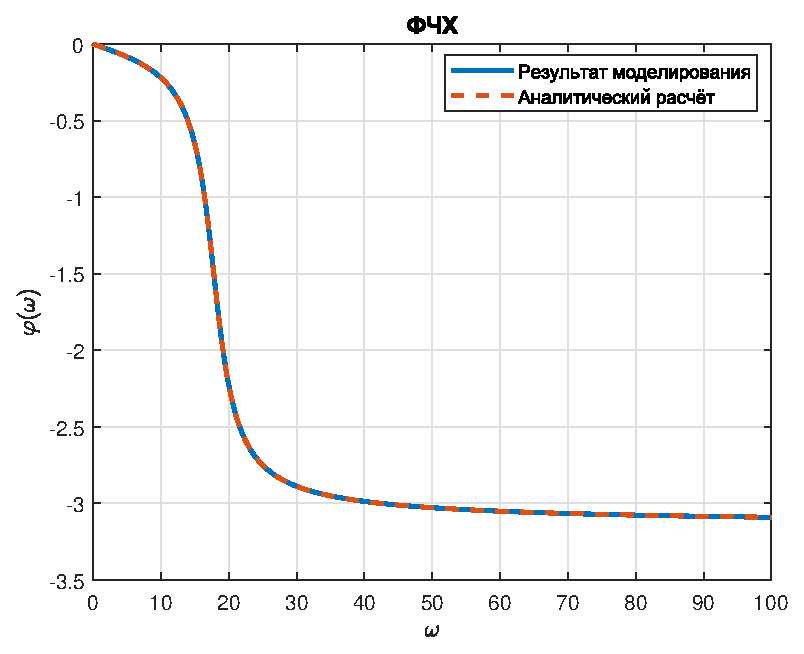
\includegraphics[width=0.65\linewidth]{ex2/fchh.eps}
    \centering
    \caption{Сравнение ФЧХ промоделированной системы с аналитически рассчитанной ФЧХ}
\end{figure}

\begin{figure}[H]
    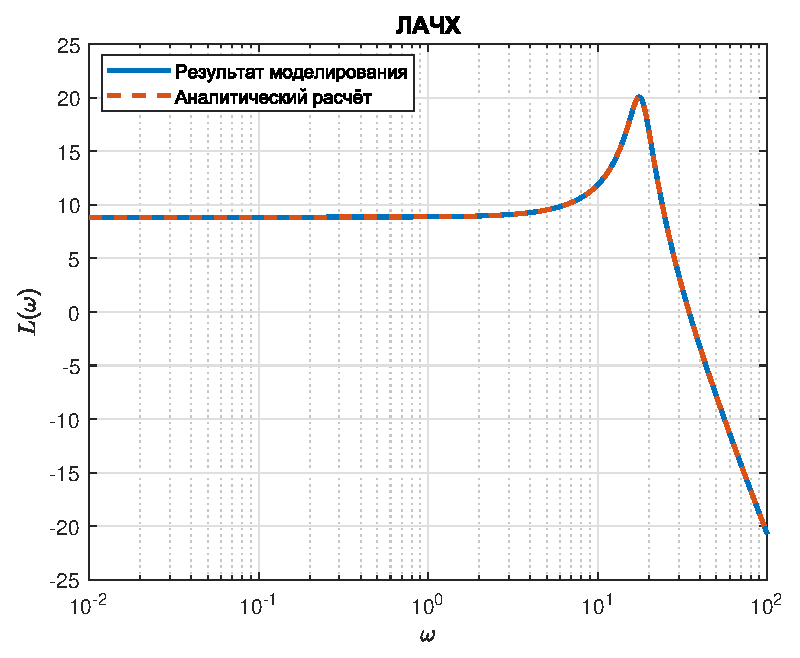
\includegraphics[width=0.65\linewidth]{ex2/lachh.eps}
    \centering
    \caption{Сравнение ЛАЧХ промоделированной системы с аналитически рассчитанной ЛАЧХ}
\end{figure}

\begin{figure}[H]
    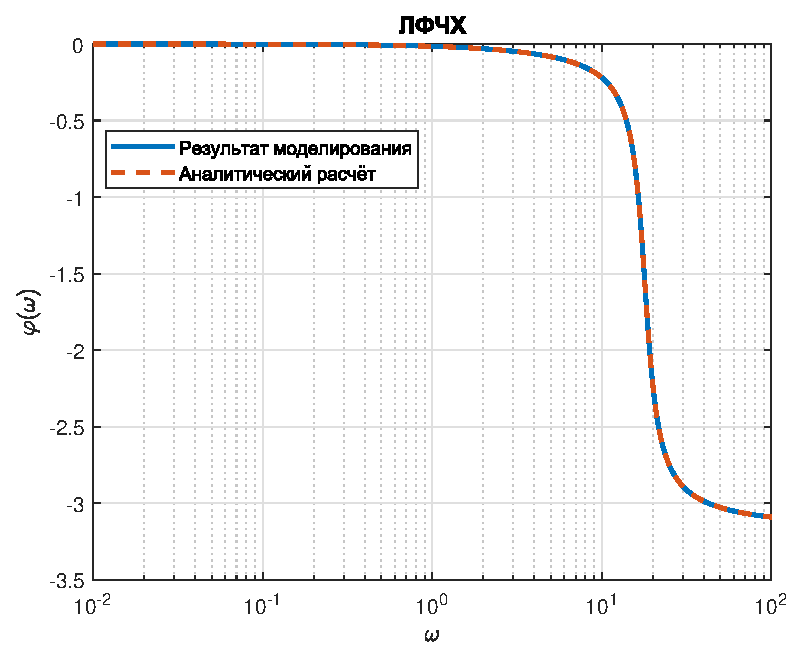
\includegraphics[width=0.65\linewidth]{ex2/lfchh.eps}
    \centering
    \caption{Сравнение ЛФЧХ промоделированной системы с аналитически рассчитанной ЛФЧХ}
\end{figure}

Результаты полученных графических представлений частотных характеристик полностью совпали с теоретическими для рассмотренного колебательного звена.

\subsubsection{Временные характеристики}\

Весовая функция:

\[
w(t) = \mathcal{L}^{-1}\left\{W(s)\right\} = \mathcal{L}^{-1}\left\{\frac{K}{T^2s^2 + 2T\xi s + 1}\right\}.
\]

Для сверки с таблицей готовых преобразований Лапласа приведу к стандартному виду с единицей в качестве коэффициента перед старшей степенью $s$:

\[
\frac{K}{T^2s^2 + 2T\xi s + 1} = \frac{K}{T^2(s^2 + \frac{2\xi}{T}s + \frac{1}{T^2})}
\]

В знаменателе можно вывести полный квадрат:

\[
T^2\left(s^2 + \frac{2\xi}{T}s + \frac{1}{T^2}\right) = T^2\left((s + \frac{\xi}{T})^2 + \frac{1-\xi^2}{T^2}\right)
\]

Для моего случая $\xi \approx 0.3445 > 0$ можно безболезненно внести замену $\frac{\xi}{T} = a, \frac{1-\xi^2}{T^2} = \omega^2$:

\[
W(s) = \frac{K}{T^2}\frac{1}{\left((s + a)^2 + \omega^2\right)}
\]

Преобразуем:

\[
\frac{1}{(s + a)^2 + \omega^2} = \frac{1}{\omega} \cdot \frac{\omega}{(s + a)^2 + \omega^2}
\]

Известно табличное преобразование Лапласа, похожее на получившееся выражение:

\[
\mathcal{L}\{\text{e}^{-at}\sin{(\omega t)}\} = \frac{\omega}{(s+a)^2+\omega^2}
\]

Так как $\frac{1}{\omega}, \frac{K}{T^2}$ --- константы, то, по свойству линейности:

\[
\mathcal{L}\left\{\frac{K}{T^2}\frac{1}{\omega}\text{e}^{-at}\sin{(\omega t)}\right\} = \frac{K}{T^2}\frac{1}{\omega}\frac{\omega}{(s+a)^2+\omega^2} = W(s).
\]

Значит,

\[
w(t) = \mathcal{L}^{-1}\left\{W(s)\right\} = \mathcal{L}^{-1}\left\{\frac{K}{T^2}\frac{1}{\omega}\frac{\omega}{(s+a)^2+\omega^2}\right\} = \frac{K}{T^2}\frac{1}{\omega}\text{e}^{-at}\sin{(\omega t)}.
\]

Подставил введённые замены $\frac{\xi}{T} = a, \frac{1-\xi^2}{T^2} = \omega^2$:

\[
w(t) = \mathcal{L}^{-1}\left\{W(s)\right\} = \frac{K}{T}\frac{1}{\frac{\sqrt{1-\xi^2}}{T}}\text{e}^{-\frac{\xi}{T}t}\sin{\left(\frac{\sqrt{1-\xi^2}}{T} t\right)} = \frac{K}{T\sqrt{1-\xi^2}}\text{e}^{-\frac{\xi}{T}t}\sin{\left(\frac{\sqrt{1-\xi^2}}{T} t\right)}.
\]

Переходная функция:

\[
y_{s.r.}(t) = \mathcal{L}^{-1}\left\{\frac{W(s)}{s}\right\}.
\]

Используя полученные при вычислении весовой функции преобразования, получаю при $a = \frac{\xi}{T}, \omega = \sqrt{\frac{1-\xi^2}{T^2}}$:

\[
\frac{W(s)}{s} = \frac{1}{s}\frac{K}{T^2}\frac{1}{\left((s + a)^2 + \omega^2\right)}.
\]

Тогда, по свойству интегрирования:

\[
y_{s.r.}(t) = \mathcal{L}^{-1}\left\{\frac{W(s)}{s}\right\} = \mathcal{L}^{-1}\left\{\frac{1}{s}\frac{K}{T^2}\frac{1}{\left((s + a)^2 + \omega^2\right)}\right\} = \int_{0^-}^{t}\frac{K}{T^2}\frac{1}{\omega}\text{e}^{-ax}\sin{(\omega x)}dx = \frac{K}{T^2\omega}\int_{0^-}^{t}\text{e}^{-ax}\sin{(\omega x)}dx
\]

Рассмотрю неопределенный интеграл $\int\text{e}^{-ax}\sin{(\omega x)}dx$:

\[
\int\text{e}^{-ax}\sin{(\omega x)}dx = \bigg[\int \text{fg}' = \text{fg} - \int \text{f}'\text{g}, \, \, f = \sin{(\omega x)}, g' = \text{e}^{-a x}\bigg] = -\frac{\text{e}^{-ax}\sin{(\omega x)}}{a} - \int - \frac{\omega\text{e}^{-ax}\cos{(\omega x)}}{a}dx.
\]

Проинтегрирую по частям ещё раз:

\[
-\frac{\text{e}^{-ax}\sin{(\omega x)}}{a} - \int - \frac{\omega\text{e}^{-ax}\cos{(\omega x)}}{a}dx = \bigg[\text{f} = \omega \cos{(\omega x), \, \, \text{g}' = -\frac{\text{e}^{-ax}}{a}}\bigg] =
\]

\[=
-\frac{\text{e}^{-ax}\sin{(\omega x)}}{a} - \left( -\frac{\omega \text{e}^{-ax}\cos{\omega x}}{a^2} - \int -\frac{\omega^2\text{e}^{-ax}\sin{(\omega x)}}{a^2} dx \right)
\]

Исходный рассматриваемый интеграл снова появляется в правой части выражения, таким образом решаем уравнение по $\int\text{e}^{-ax}\sin{(\omega x)}dx$:

\[
F(x) = -\frac{\text{e}^{-ax} \left(a \sin\left({\omega}x\right) + \omega \cos\left(\omega x\right)\right)}{{\omega}^{2} + a^{2}} + C
\]

Первообразная найдена, можно посчитать определенный интеграл:

\[
y_{s.r.}(t) = \frac{K}{T^2\omega}\int_{0^-}^{t}\text{e}^{-ax}\sin{(\omega x)}dx = F(t) - F(0^-) = \frac{K}{T^2\omega}\left(\frac{\omega}{{\omega}^{2} + a^{2}} - \frac{a \sin\left(t{\omega}\right) + {\omega} \cos\left(t{\omega}\right)}{\mathrm{e}^{at} {\omega}^{2} + a^{2} \mathrm{e}^{at}}\right) = 
\]

\[=
\frac{K}{T^2\omega({\omega}^{2} + a^{2})}\left(\omega - \text{e}^{-at}(a \sin\left(t{\omega}\right) + {\omega} \cos\left(t{\omega}\right))\right)
\]

Произведу обратную замену $a = \frac{\xi}{T}, \omega = \frac{\sqrt{1-\xi^2}}{T}$:

\[
y_{s.r.}(t) = \frac{K}{T^2\frac{\sqrt{1-\xi^2}}{T}\left(\left({\frac{\sqrt{1-\xi^2}}{T}}\right)^{2} + \left(\frac{\xi}{T}\right)^{2}\right)}\left(\frac{\sqrt{1-\xi^2}}{T} - \text{e}^{-\frac{\xi t}{t}}\left(\frac{\xi}{T} \sin\left(t{\frac{\sqrt{1-\xi^2}}{T}}\right) + {\frac{\sqrt{1-\xi^2}}{T}} \cos\left(t{\frac{\sqrt{1-\xi^2}}{T}}\right)\right)\right) = 
\]

\[=
\frac{K}{\cancel{T}\cancel{\sqrt{1-\xi^2}}\left({\frac{1-\xi^2 + \xi^2}{\cancel{T^2}}}\right)}\frac{\cancel{\sqrt{1-\xi^2}}}{\cancel{T}}\left(1 - \text{e}^{-\frac{\xi t}{T}}\left(\frac{\xi}{\cancel{T}}\frac{{\cancel{T}}}{\sqrt{1-\xi^2}} \sin\left(t{\frac{\sqrt{1-\xi^2}}{T}}\right) + \cos\left(t{\frac{\sqrt{1-\xi^2}}{T}}\right)\right)\right) = 
\]

\[
= K\left(1 - \text{e}^{-\frac{\xi t}{T}}\left(\frac{\xi}{\sqrt{1-\xi^2}} \sin\left(t{\frac{\sqrt{1-\xi^2}}{T}}\right) + \cos\left(t{\frac{\sqrt{1-\xi^2}}{T}}\right)\right)\right).
\]

Подставлю исходные данные в полученные функции:

\[
w(t) = \frac{K}{T\sqrt{1-\xi^2}}\text{e}^{-\frac{\xi}{T}t}\sin{\left(\frac{\sqrt{1-\xi^2}}{T} t\right)} = 19.1327\text{e}^{-2.2356t}\sin{(6.0921 t)}
\]

\[
y_\text{s.r.}(t) = K\left(1 - \text{e}^{-\frac{\xi t}{T}}\left(\frac{\xi}{\sqrt{1-\xi^2}} \sin\left(t{\frac{\sqrt{1-\xi^2}}{T}}\right) + \cos\left(t{\frac{\sqrt{1-\xi^2}}{T}}\right)\right)\right)=
\]

\[
= 2.7685\bigg(1 - e^{-2.2356t}\big(0.3669\sin{(6.0921t)}+ \cos{(6.0921t)}\big)\bigg).
\]

\subsubsection*{Моделирование}\

Снова проведя моделирование, я получил временные характеристики системы, и сопоставил их с полученными аналитически:

\begin{figure}[H]
    \includegraphics[width=0.65\linewidth]{ex2/step.eps}
    \centering
    \caption{Сравнение промоделированной переходной функции с полученной аналитически}
\end{figure}

\begin{figure}[H]
    \includegraphics[width=0.65\linewidth]{ex2/impulse.eps}
    \centering
    \caption{Сравнение промоделированной весовой функции с полученной аналитически}
\end{figure}

Результаты полученных графических представлений временных характеристик полностью совпали с теоретическими для рассмотренного колебательного звена.

\subsection{Конденсируй-умножай}\

В задании рассматривается уравнение конденсатора 

\[
I = C \frac{dU}{dt}
\]
с $I(t)$ в качестве входа и $U(t)$ в качестве выхода.

Для вывода передаточной функции представлю уравнение в виде

\[
C\dot U = I
\]

Тогда передаточная функция выглядит следующим образом:

\[
W(s) = \frac{1}{Cs}
\]

Она представима в стандартизированной форме:

\[
W(s) = \frac{K}{s}, K = \frac{1}{C}
\]

Функция сопоставима с идеальным интегрирующим звеном. Ёмкость конденсатора --- величина неотрицательная, соответственно и $K > 0$. 

\subsubsection{Частотные характеристики}\

Для определения АЧХ и ФЧХ перейду к частотной передаточной функции и разобью её на вещественную и мнимую составляющие:

\[
W(s) = \frac{K}{s} \Leftrightarrow W(j\omega) = \frac{K}{j\omega}
\]

\[
W(j\omega) = \frac{-jK\omega}{(j\omega)(-j\omega)} = \frac{-jK\omega}{\omega^2} = \frac{-jK}{\omega}.
\]

В этом случае действительная составляющая $P(\omega)$ равна $0$, значит, $W(j\omega) = P(\omega) + jQ(\omega)$ --- чисто мнимое число, при этом $Q(\omega) < 0$. Найду АЧХ:

\[
A(\omega) = \sqrt{W(j\omega)^2} = \sqrt{\left(\frac{-jK}{\omega}\right)^2} = \frac{K}{\omega}.
\]

Тогда ЛАЧХ:

\[
L(\omega) = 20 \lg A(\omega) = 20 \lg \left( \frac{K}{\omega} \right)
\]

Разложим логарифм:

\[
L(\omega) = 20 \lg K - 20 \lg \omega.
\]

ФЧХ же в этом случае будет определяться так:

\[
\varphi(\omega) = \text{atan2}\left(\frac{-K}{\omega}, 0\right) = -\frac{\pi}{2}.
\]

Подставляя значения исходных данных для своего варианта, получаю 

\[
K = \frac{1}{C} = \frac{1}{314} \approx 0.0032\Rightarrow W(s) = \frac{0.0032}{s}.
\]

\[
A(\omega) = \frac{K}{\omega} = \frac{0.0032}{\omega}.
\]

\[
L(\omega) = 20 \lg \left(\frac{0.0032}{\omega}\right).
\]

\subsubsection*{Моделирование}\

Полученная передаточная функция была промоделирована, и результаты моделирования были сопоставлены с полученными аналитически:

\begin{figure}[H]
    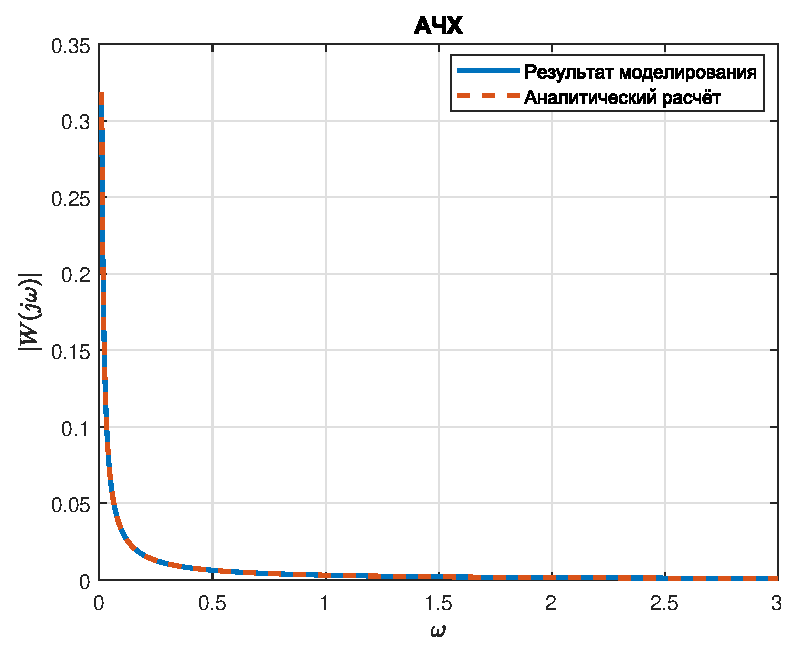
\includegraphics[width=0.65\linewidth]{ex3/achh.eps}
    \centering
    \caption{Сравнение АЧХ промоделированной системы с аналитически рассчитанной АЧХ}
\end{figure}

\begin{figure}[H]
    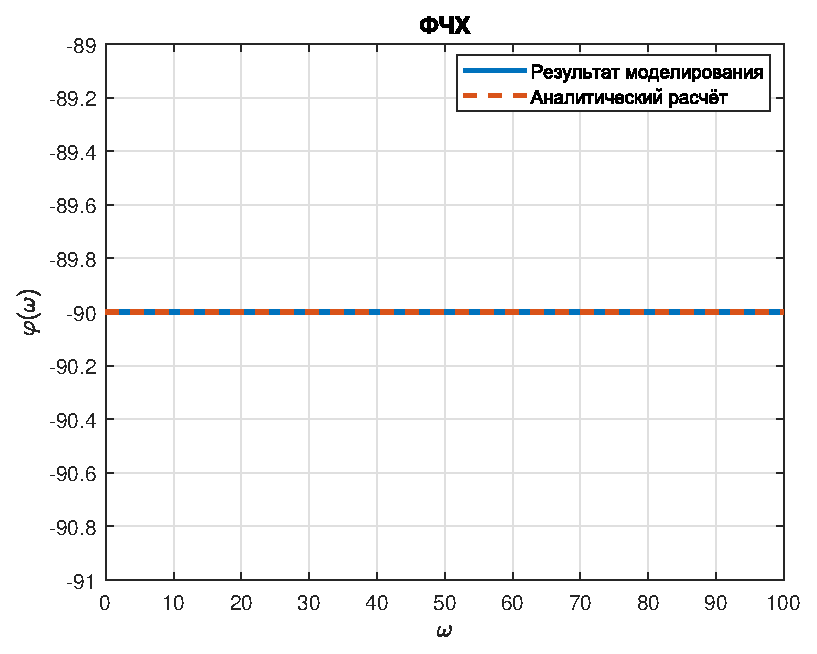
\includegraphics[width=0.65\linewidth]{ex3/fchh.eps}
    \centering
    \caption{Сравнение ФЧХ промоделированной системы с аналитически рассчитанной ФЧХ}
\end{figure}

\begin{figure}[H]
    \includegraphics[width=0.65\linewidth]{ex3/lachh.eps}
    \centering
    \caption{Сравнение ЛАЧХ промоделированной системы с аналитически рассчитанной ЛАЧХ}
\end{figure}

\begin{figure}[H]
    \includegraphics[width=0.65\linewidth]{ex3/lfchh.eps}
    \centering
    \caption{Сравнение ЛФЧХ промоделированной системы с аналитически рассчитанной ЛФЧХ}
\end{figure}

Результаты полученных графических представлений частотных характеристик полностью совпали с теоретическими для рассмотренного идельного интегрирующего звена.

\subsubsection{Временные характеристики}\ 

Весовая функция для уравнения конденсатора:

\[
w(t) = \mathcal{L}^{-1}\{W(s)\} = \mathcal{L}^{-1}\left\{\frac{K}{s}\right\} = K\cdot\mathcal{L}^{-1}\left\{\frac{1}{s}\right\} = K
\]

Переходная функция:

\[
y_{s.r.}(t) = \mathcal{L}^{-1}\left\{\frac{W(s)}{s}\right\} = \mathcal{L}^{-1}\left\{\frac{K}{s^2}\right\} = K\cdot\mathcal{L}^{-1}\left\{\frac{1}{s^2}\right\} = Kt
\]

Подставляя исходные данные для этого объекта, получаю:

\[
w(t) = K = 0.0032,
\]

\[
y_\text{s.r.}(t) = Kt = 0.0032t.
\]

\subsubsection*{Моделирование}\

Снова проведя моделирование, я получил временные характеристики системы, и сопоставил их с полученными аналитически:

\begin{figure}[H]
    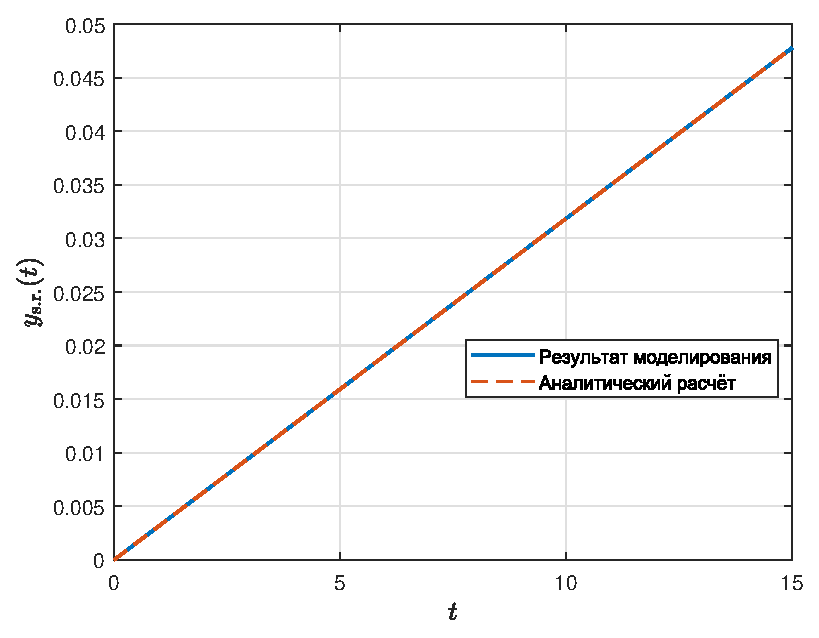
\includegraphics[width=0.65\linewidth]{ex3/step.eps}
    \centering
    \caption{Сравнение промоделированной переходной функции с полученной аналитически}
\end{figure}

\begin{figure}[H]
    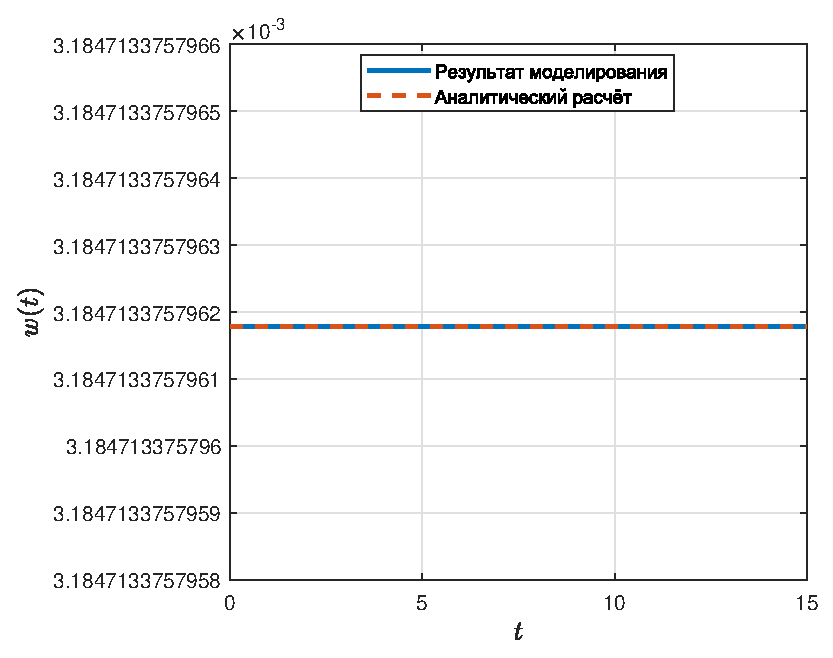
\includegraphics[width=0.65\linewidth]{ex3/impulse.eps}
    \centering
    \caption{Сравнение промоделированной весовой функции с полученной аналитически}
\end{figure}

Результаты полученных графических представлений временных характеристик полностью совпали с теоретическими для рассмотренного идеального интегрирующего звена.

\subsection{Пружинка}\

В задании рассматривается пружинный маятник, представленный на рисунке:

\begin{figure}[H]
    \centering
    \includegraphics[width=0.5\linewidth]{ex4/scheme.png}
    \caption{Пружинный маятник}
\end{figure}\

Его движение задаётся следующими уравнениями:

\[
F_\text{упр} = -kx, F = ma.
\]

Входом этой системы считается некая внешняя сила $F_\text{ext}$, направленная соосно движению маятника, а выходом --- траектория движения $x(t)$. Так как $a = \ddot x$:

\[
F_{ext}(t) = m \ddot{x} + k x
\]

Переходим к пространству изображений Лапласа:

\[
m s^2 X(s) + k X(s) = F_{\text{ext}}(s)
\]

\[
X(s) \left(m s^2 + k\right) = F_{\text{ext}}(s)
\]

\[
W(s) = \frac{X(s)}{F_{\text{ext}}(s)} = \frac{1}{m s^2 + k} = \frac{1}{k}\frac{1}{\frac{m}{k}s^2 + 1}
\]

В стандартизированной форме:

\[
W(s) = \frac{K}{T^2s^2+1}, K = \frac{1}{k}, T^2 = \frac{m}{k}
\]

Получаем консервативное звено. 

\subsubsection{Частотные характеристики}\

Найдём АЧХ и ФЧХ, перейдя к частотной передаточной функции:

\[
W(s) = \frac{K}{T^2s^2+1} \Rightarrow W(j\omega) = \frac{K}{T^2(j\omega)^2+1} = \frac{K}{-T^2\omega^2+1}
\]

В этом случае в качестве $W(j\omega)$ получается вещественное число. Тогда АЧХ --- просто его модуль:

\[
A(\omega) = \left|W(j\omega)\right| = \left|\frac{K}{-T^2\omega^2+1}\right|.
\]

ЛАЧХ:

\[
L(\omega) = 20 \lg A(\omega) = 20 \lg \left| \frac{K}{1 - T^2 \omega^2} \right|
= 20 \lg K - 20 \lg \left| 1 - T^2 \omega^2 \right|.
\]

Заметно, что АЧХ имеет разрыв в точке $\omega_0 = \frac{1}{T}$, и ФЧХ также не определена на этой частоте из-за наличия резонанса (знаменатель становится равен нулю). При этом частотная передаточная функция положительна, если $0 < \omega \leq \omega_0$, и отрицательна при $\omega > \omega_0$. Имея $Q(\omega) = 0, P(\omega) = \frac{K}{-T^2\omega^2+1}$, получаем:

\[
\text{atan2}(Q(\omega), P(\omega)) = \arctan{\left(\frac{0}{P(\omega)}\right)} = 0.
\]

\[
\begin{cases}
    0, & 0 < \omega \leq \frac{1}{T} \\
    -\pi, & \omega > \frac{1}{T}.
\end{cases}
\]

Подставляя значения исходных данных для своего варианта, получаю 

\[
K = \frac{1}{k} = \frac{1}{324} \approx 0.0031, T = \sqrt{\frac{m}{k}} = \sqrt{\frac{35}{324}} \approx 0.3287 \Rightarrow W(s) = \frac{0.0031}{0.1081s^2 + 1}
\]

\[
A(\omega) = \left|\frac{0.0031}{0.1081s^2 + 1}\right| = \frac{0.0031}{0.1081s^2 + 1}.
\]

\[
L(\omega) = 20 \lg \left(\frac{0.0031}{0.1081s^2 + 1}\right)
\]

\[
\varphi(\omega) = 
\begin{cases}
    0, & 0 < \omega \leq 3.0423, \\
    -\pi, & \omega > 3.0423.
\end{cases}\
\]

\subsubsection*{Моделирование}\

Полученная передаточная функция была промоделирована, и результаты моделирования были сопоставлены с полученными аналитически:

\begin{figure}[H]
    \includegraphics[width=0.65\linewidth]{ex4/achh.eps}
    \centering
    \caption{Сравнение АЧХ промоделированной системы с аналитически рассчитанной АЧХ}
\end{figure}

\begin{figure}[H]
    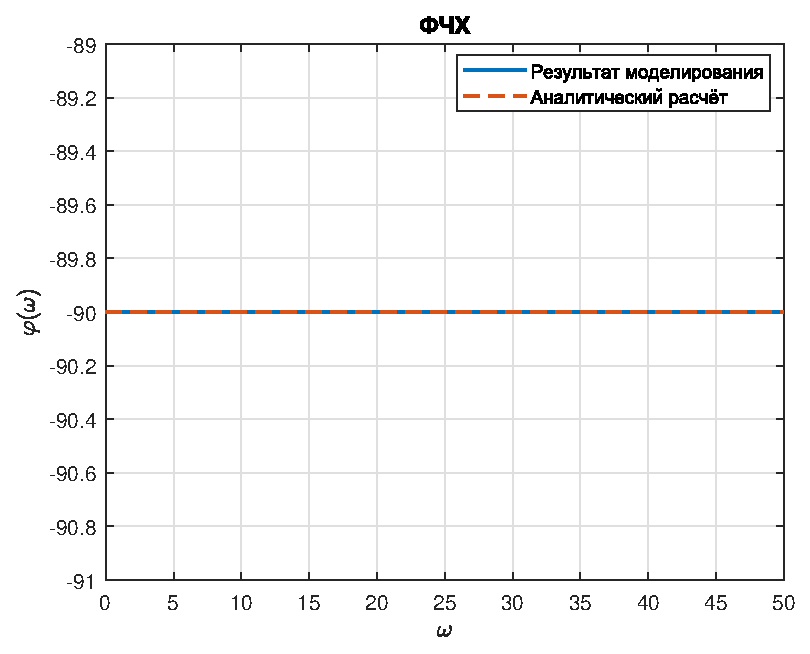
\includegraphics[width=0.65\linewidth]{ex4/fchh.eps}
    \centering
    \caption{Сравнение ФЧХ промоделированной системы с аналитически рассчитанной ФЧХ}
\end{figure}

\begin{figure}[H]
    \includegraphics[width=0.65\linewidth]{ex4/lachh.eps}
    \centering
    \caption{Сравнение ЛАЧХ промоделированной системы с аналитически рассчитанной ЛАЧХ}
\end{figure}

\begin{figure}[H]
    \includegraphics[width=0.65\linewidth]{ex4/lfchh.eps}
    \centering
    \caption{Сравнение ЛФЧХ промоделированной системы с аналитически рассчитанной ЛФЧХ}
\end{figure}

Результаты полученных графических представлений частотных характеристик полностью совпали с теоретическими для рассмотренного консервативного звена.

\subsubsection{Временные характеристики}\

Для поиска весовой функции сведу передаточную функцию до табличного значения:

\[
W(s) = \frac{K}{T^2 s^2 + 1} = \frac{K}{T^2} \cdot \frac{1}{s^2 + \frac{1}{T^2}} = \frac{K}{T} \cdot \frac{1/T}{s^2 + (1/T)^2}
\]

\[
w(t) = \mathcal{L}^{-1}\left\{ \frac{\omega}{s^2 + \omega^2} \right\} = \sin(\omega t) \Rightarrow w(t) = \frac{K}{T} \sin\!\left( \frac{t}{T} \right)
\]

Переходная функция:

\[
w_{s.r}(t) = \mathcal{L}^{-1}\left\{ \frac{W(s)}{s} \right\} = \mathcal{L}^{-1}\left\{ \frac{K}{s(T^2 s^2 + 1)} \right\}
\]

Разложу на элементарные дроби:

\[
\frac{K}{s(T^2 s^2 + 1)} = K \left( \frac{1}{s} - s\frac{T^2}{T^2 s + 1} \right)
\]

\(\mathcal{L}^{-1}\{1/s\} = 1\), \(\mathcal{L}^{-1}\left\{ s\dfrac{1}{s + (1/T)^2} \right\} = \cos{\left( \dfrac{t}{T} \right)}\), тогда:

\[
w_{s.r}(t) = K\mathcal{L}^{-1}\left\{ \frac{1}{s} - \frac{T^2 s}{T^2 s^2 + 1} \right\} = K\left(1 - \cos\!\left( \frac{t}{T} \right)\right).
\]

Подставлю исходные данные:

\[
w(t) = \frac{K}{T}\sin{\left(\frac{t}{T}\right)} = 0.0094\sin{\left(\frac{t}{0.3287}\right)}.
\]

\[
y_\text{s.r.}(t) = K\left(1-\cos{\left(\frac{t}{T}\right)}\right) = 0.0031\left(1-\cos{\left(\frac{t}{0.3287}\right)}\right)
\]

\subsubsection*{Моделирование}\

Снова проведя моделирование, я получил временные характеристики системы, и сопоставил их с полученными аналитически:

\begin{figure}[H]
    \includegraphics[width=0.65\linewidth]{ex4/step.eps}
    \centering
    \caption{Сравнение промоделированной переходной функции с полученной аналитически}
\end{figure}

\begin{figure}[H]
    \includegraphics[width=0.65\linewidth]{ex4/impulse.eps}
    \centering
    \caption{Сравнение промоделированной весовой функции с полученной аналитически}
\end{figure}

Результаты полученных графических представлений временных характеристик полностью совпали с теоретическими для рассмотренного консервативного звена.

\subsection{Что ты такое?}\

В задании рассматривается схема регулятора на операционном усилителе, представленная на рисунке:

\begin{figure}[H]
    \centering
    \includegraphics[width=0.65\linewidth]{ex5/scheme.png}
    \caption{Принципиальная схема регулятора на операционном усилителе}
\end{figure}\

Считая входом системы $U_\text{ВХ}(t)$, а выходом --- $U_\text{ВЫХ}(t)$, можем рассмотреть преобразования, выполняемые над входным сигналом более подробно:\

На входном резисторе сопротивлением $R_1$ при подаче напряжения появляется ток $I(t) = \frac{U_\text{ВХ}(t)}{R_1}$. Далее этот ток попадает на конденсатор с отрицательной обратной связью ёмкостью $C$, и, зная что ток, проходящий через конденсатор такой ёмкости, равен $I(t) = C\frac{du(t)}{dt}$, можем рассчитать напряжение на нём: 

\[
u(t) = u(0) + \frac{1}{C}\int_0^{t} I(x)dx.
\]

Воспользуемся полученным ранее значением $I(t) = \frac{U_\text{ВХ}(t)}{R_1}$ и примем начальное условие $u(0) = 0$, тогда $u(t) = \frac{1}{C}\int_0^{t} \frac{U_\text{ВХ}(x)}{R_1}dx = \frac{1}{R_1C}\int_0^{t} U_\text{ВХ}(x)dx$. В пространстве изображений Лапласа по свойству интегрирования после прохождения конденсатора выходом будет являться $Z(s) = \frac{1}{R_1Cs}$ Далее сигнал идёт на последовательно подключенный резистор $R_2$, и выходом по обратной связи будет являться $W(s) = \frac{1}{R_1Cs} + R_2\cdot I(s) = \frac{1}{R_1Cs} + \frac{R_2}{R_1} = \frac{1 + R_2 Cs}{R_1 Cs}$.

Получается изодромное звено. Так как передаточная функция этого регулятора состоит из двух слагаемых, интегрирующего $\frac{1}{R_1Cs}$ и пропорционального $\frac{R_2}{R_1}$, то регулятор пропорционально-интегральный (ПИ).

Передаточная функция объекта найдена, можно привести её к стандартизированной форме:

\[
W(s) = \frac{1 + R_2 Cs}{R_1 Cs} = \frac{1}{R_1C}\frac{R_2Cs + 1}{s} = \frac{K(Ts + 1)}{s}, K = \frac{1}{R_1C}, T = R_2C.
\]

\subsubsection{Частотные характеристики}\

Для нахождения АЧХ и ФЧХ переведу уравнение в частотную область:

\[
W(s) = \frac{K(Ts + 1)}{s} \Rightarrow W(j\omega) = \frac{K(T(j\omega) + 1)}{(j\omega)}
\]

Домножу числитель и знаменатель на сопряженное:

\[
W(j\omega) = \frac{K(-T(j\omega)^2 - (j\omega))}{-(j\omega)(j\omega)} = \frac{KT\omega^2 - jK\omega}{\omega^2} = \frac{KT\omega^2}{\omega^2} + j\frac{-K\omega}{\omega^2} = KT + j\frac{-K}{\omega}
\]

Пусть $P(\omega) = KT$, $Q(\omega) = -\frac{K}{\omega}$. Тогда АЧХ:

\[
A(\omega) = \sqrt{P(\omega)^2 + Q(\omega)^2} = \sqrt{K^2T^2 + \frac{K^2}{\omega^2}} = K\sqrt{T^2 + \frac{1}{\omega^2}}
\]

ЛАЧХ определяется как:

\[
L(\omega) = 20 \lg A(\omega) = 20 \lg \left( K \sqrt{T^2 + \frac{1}{\omega^2}} \right)
\]

\[
= 20 \lg K + 20 \lg \left( \sqrt{T^2 + \frac{1}{\omega^2}} \right)
= 20 \lg K + 10 \lg \left( T^2 + \frac{1}{\omega^2} \right).
\]

Также вычислю и ФЧХ:

\[
\varphi(\omega) = \text{atan2}(Q(\omega), P(\omega) = \text{atan2}\left(-\frac{K}{\omega}, KT\right))
\]

$K = \frac{1}{R_1C} > 0$, так как сопротивление резистора и ёмкость конденсатора --- величины положительные. $T = R_2C > 0$ по той же причине, а значит, $Q(\omega) = -\frac{K}{\omega} < 0 \ \,\forall \ \omega > 0$, и $P(\omega) = KT > 0$. Следовательно, $W(\omega) = P(\omega) + jQ(\omega)$ всегда расположено во втором квадранте. В этом случае $\text{atan2}(Q(\omega), P(\omega)) = \arctan{\left(\frac{Q(\omega)}{P(\omega)}\right)}$. Тогда:

\[
\varphi(\omega) = \arctan{\left(\frac{Q(\omega)}{P(\omega)}\right)} = \arctan{\left( \frac{-\frac{K}{\omega}}{KT}\right)} = \arctan{\left(\frac{-1}{T\omega}\right)} = \arctan{\left(\frac{-1}{T\omega}\right)} = \arctan{\left(\frac{1}{T\omega}\right)}.
\]

Подставляя значения исходных данных для своего варианта, получаю 

\[
K = \frac{1}{R_1 C} = \frac{1}{6427\cdot314} \approx 4.955\cdot10^{-7}, T = R_2C = 19282 \cdot 314 = 6054548 \Rightarrow W(s) = \frac{4.955\cdot10^{-7}(6054548s + 1)}{s}.
\]

\[
A(\omega) = K\sqrt{T^2 + \frac{1}{\omega^2}} = 4.955\cdot10^{-7}\sqrt{6054548^2 + \frac{1}{\omega^2}}.
\]

\[
L(\omega) = 20 \lg \left(4.955\cdot10^{-7}\sqrt{6054548^2 + \frac{1}{\omega^2}}\right)
\]

\[
\varphi(\omega) = \text{arctan}\left(\frac{1}{6054548\omega}\right).
\]

\subsubsection*{Моделирование}\

Полученная передаточная функция была промоделирована, и результаты моделирования были сопоставлены с полученными аналитически:

\begin{figure}[H]
    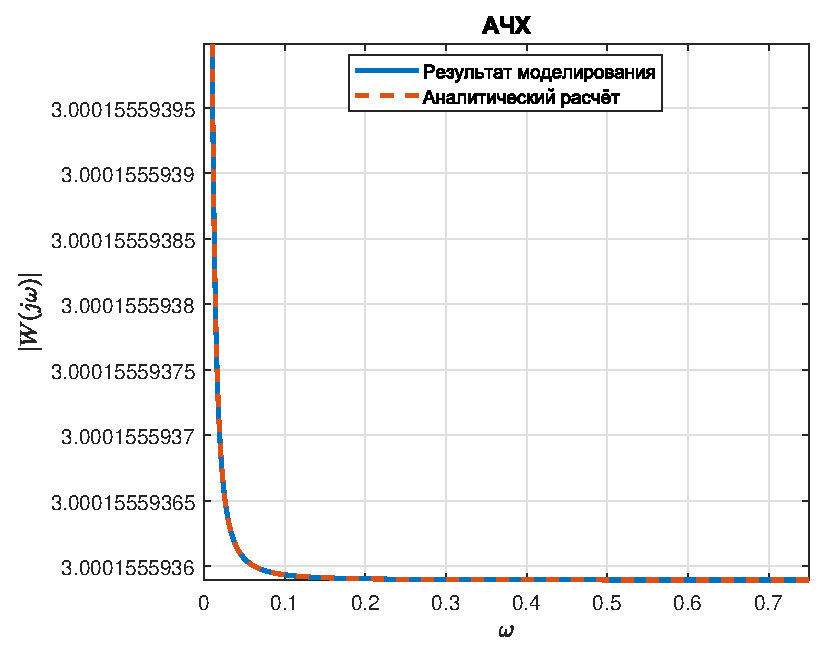
\includegraphics[width=0.65\linewidth]{ex5/achh.eps}
    \centering
    \caption{Сравнение АЧХ промоделированной системы с аналитически рассчитанной АЧХ}
\end{figure}

\begin{figure}[H]
    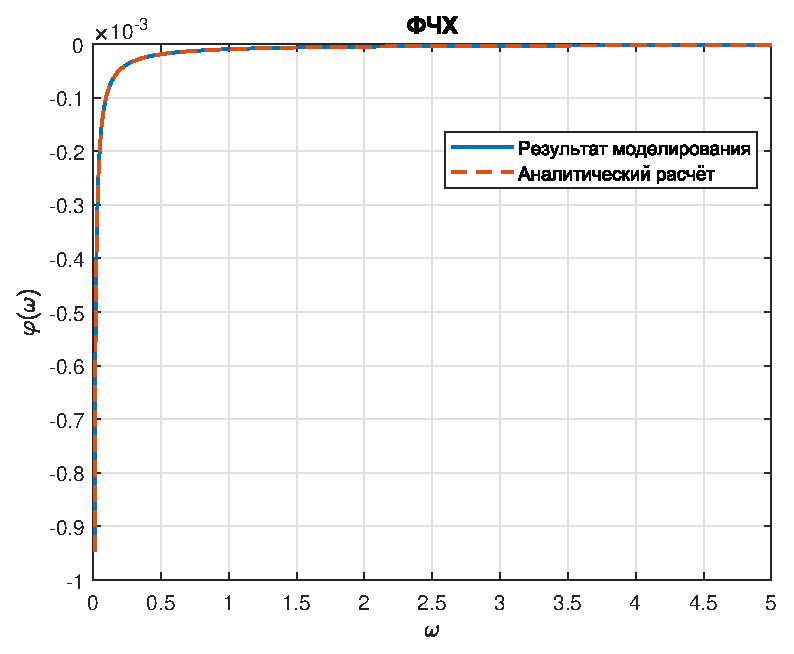
\includegraphics[width=0.65\linewidth]{ex5/fchh.eps}
    \centering
    \caption{Сравнение ФЧХ промоделированной системы с аналитически рассчитанной ФЧХ}
\end{figure}

\begin{figure}[H]
    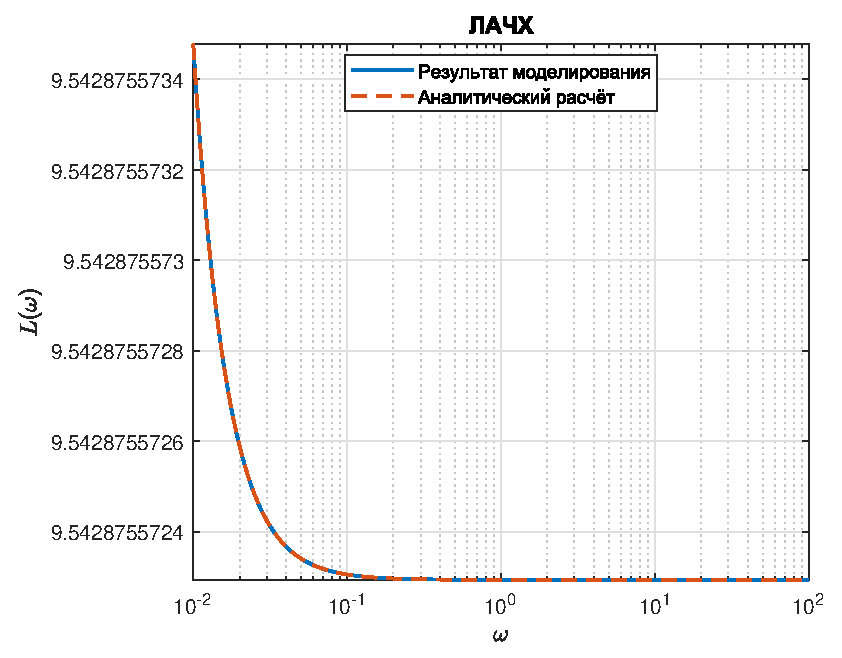
\includegraphics[width=0.65\linewidth]{ex5/lachh.eps}
    \centering
    \caption{Сравнение ЛАЧХ промоделированной системы с аналитически рассчитанной ЛАЧХ}
\end{figure}

\begin{figure}[H]
    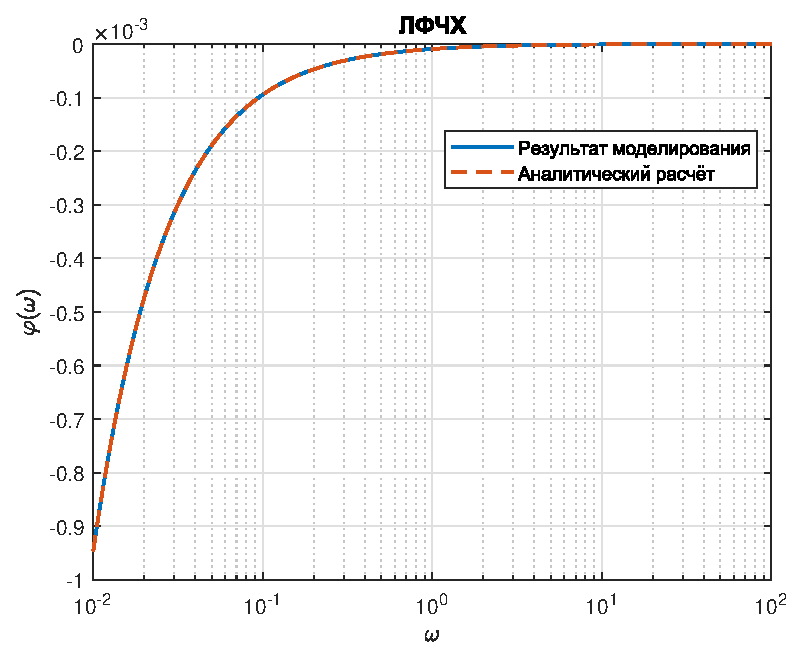
\includegraphics[width=0.65\linewidth]{ex5/lfchh.eps}
    \centering
    \caption{Сравнение ЛФЧХ промоделированной системы с аналитически рассчитанной ЛФЧХ}
\end{figure}

Результаты полученных графических представлений частотных характеристик полностью совпали с теоретическими для рассмотренного изодромного звена.

\subsubsection{Временные характеристики}\

Разложу передаточную функцию для удобного нахождения весовой функции:

\[
W(s) = \frac{K(Ts + 1)}{s} = KT + \frac{K}{s}
\]

\[
w(t) = \mathcal{L}^{-1}\{W(s)\} = KT\,\delta(t)  + K
\]

Передаточная функция $y_{s.r.}(t)$ всё также является реакцией системы на единичный скачок, образ Лапласа которого --- $\frac{1}{s}$:

\[
y_{s.r.}(t) = \mathcal{L}^{-1}\left\{ \frac{W(s)}{s} \right\}
\]

\[
\frac{W(s)}{s} = \frac{K(Ts + 1)}{s^2} = K \left( \frac{T}{s} + \frac{1}{s^2} \right)
\]

\(\mathcal{L}^{-1}\{1/s\} = 1\), \(\mathcal{L}^{-1}\{1/s^2\} = t\), следовательно:

\[
y_{s.r.}(t) = K\bigl( T + t \bigr)
\]

В очередной раз подставлю исходные данные и найду характеристики для объекта с ними:

\[
w(t) = KT\,\delta(t) + K = 3.001\delta(t) + 4.955\cdot10^{-7},
\]

\[
y_\text{s.r.}(t) = 3.001 + 4.955\cdot10^{-7}t.
\]

\subsubsection*{Моделирование}\

Снова проведя моделирование, я получил временные характеристики системы, и сопоставил их с полученными аналитически:

\begin{figure}[H]
    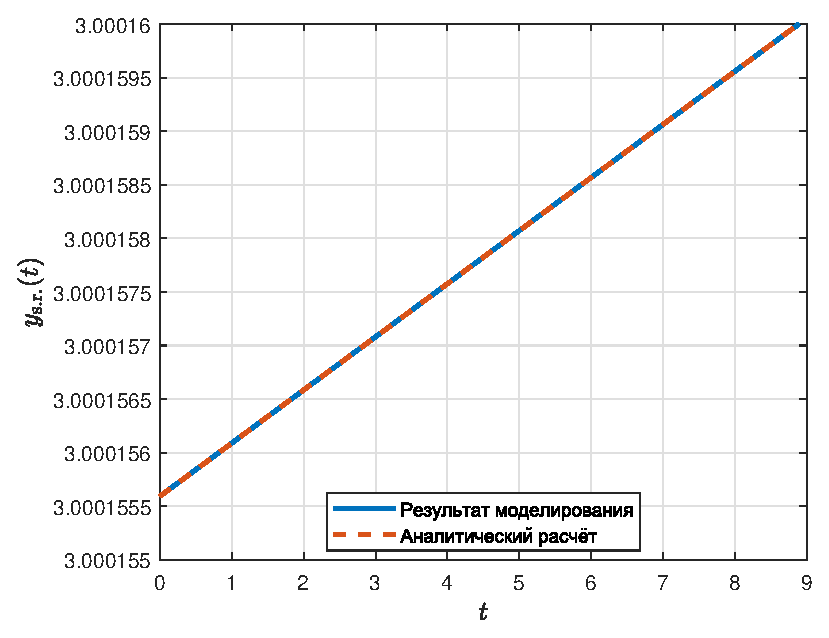
\includegraphics[width=0.65\linewidth]{ex5/step.eps}
    \centering
    \caption{Сравнение промоделированной переходной функции с полученной аналитически}
\end{figure}

\begin{figure}[H]
    \includegraphics[width=0.65\linewidth]{ex5/impulse.eps}
    \centering
    \caption{Сравнение промоделированной весовой функции с полученной аналитически}
\end{figure}

Результаты полученных графических представлений временных характеристик полностью совпали с теоретическими для рассмотренного изодромного звена.

\section{Вывод по работе}\ 

В ходе работы я ознакомился с основными типовыми звеньями, их частотными и временными характеристиками, научился вычислять их аналитически, проверил полученные результаты программным моделированием.

\section{Приложение А. Код для выполнения заданий}

\subsection*{Листинг 1. Код для выполнения заданий}

\begin{lstlisting}[caption={Код для построения графиков характеристик для всех рассмотренных объектов}, language=matlab]
clear all;
close all;

[~, scriptName] = fileparts(mfilename('fullpath'));
if ~isfolder(scriptName)
    mkdir(scriptName);
end

km = 0.3612;
ke = 0.3612;
J = 0.0031;
R = 4.7237;
L = 1.0567;

N = 1000;
w = logspace(-2, 2, N);  % от 0.01 до 100 рад/с
s = 1j * w;

t_final = 15; % время моделирования 
t = linspace(0, t_final, 1000);

% K = 1 / ke;
% T = (J * R) / (ke * km);
% A = K ./ sqrt((1 + (T.*w).^2));
% L = 20*log10(K) - 10*log10(1 + (T.*w).^2);
% phi = atan2(((-K * T) .* w)./(1 + (T.*w).^2), (K)./(1 + (T.*w).^2));
% phi = rad2deg(phi);
% num = K;
% den = [T, 1];
% sys = tf(num, den)                   % дпт
% [mag, phase, wout] = bode(sys, w);
% mag = squeeze(mag);
% phase = squeeze(phase);
% y_imp_native = (K / T) .* exp((-1/T) .* t);
% y_step_native = K * (1 - exp(-t .* (1/T)));
% [y_imp, t_imp] = impulse(sys, t);
% [y_step, t_step] = step(sys, t);


% K = 1 / ke;
% T = sqrt((J) / ke * km);
% xi = (T * R) / 2 * L;
% A = K * sqrt( (T^2 * w.^2 .* (4*xi^2 - 2 + T^2 * w.^2) + 1) ./ ((1 - T^2 * w.^2).^2 + (2*T*xi*w).^2).^2);
% L = 20*log10(A);
% phi = zeros(size(w));
% idx1 = w < 1/T;
% idx2 = w > 1/T;
% idx_eq = abs(w - 1/T) < 1e-12;
% phi(idx1) = -atan( (2*T*xi*w(idx1)) ./ (1 - T^2 * w(idx1).^2) );
% phi(idx_eq) = -pi/2;
% phi(idx2) = -atan( (2*T*xi*w(idx2)) ./ (1 - T^2 * w(idx2).^2) ) - pi;
% phi = rad2deg(phi);
% 
% num = K;
% den = [T^2, 2*T*xi, 1];
% sys = tf(num, den)                   % DPT 2.0
% [mag, phase, wout] = bode(sys, w);
% mag = squeeze(mag);
% phase = squeeze(phase);
% % W = K ./ (T^2 * s.^2 + 2*T*xi*s + 1); % DPT 2.0
% y_imp_native = (K / (T*sqrt(1-xi^2))) .* exp((-xi/T) .* t) .* sin(((sqrt(1-xi^2))/T).*t);
% y_step_native = K * (1 - exp(-(xi .* t)/T) .* ( (xi ./ sqrt(1 - xi^2)) .* sin(t .* (sqrt(1 - xi^2) / T)) + cos(t .* (sqrt(1 - xi^2) / T)) ));
% [y_imp, t_imp] = impulse(sys, t);
% [y_step, t_step] = step(sys, t);



% K = 1 / 314;
% A = K ./ w;
% L = 20 * log10(K) - 20 .* log10(w);
% phi = (-pi / 2) .* ones(size(w));
% phi = rad2deg(phi);
% 
% num = K;
% den = [1, 0];
% sys = tf(num, den)                   % конденсируй-умножай
% [mag, phase, wout] = bode(sys, w);
% mag = squeeze(mag);
% phase = squeeze(phase);
% 
% % W = K ./ (s);                         % конденсируй-умножай
% y_imp_native = K .* ones(size(t));
% y_step_native = K .* t;
% [y_imp, t_imp] = impulse(sys, t);
% [y_step, t_step] = step(sys, t);


% M = 35;
% k = 324;
% K = 1 / k;
% T = sqrt(M / k);
% A = abs(K ./ (-T^2 .* w.^2 + 1));
% L = 20 * log10(K) - 20 * log10(abs(1 - (T^2).*(w.^2)));
% phi = zeros(size(w));
% idx1 = w <= 1/T;
% idx2 = w > 1/T;
% phi(idx1) = 0;
% phi(idx2) = -pi;
% phi = rad2deg(phi);
% 
% num = K;
% den = [T^2, 0, 1];
% sys = tf(num, den)                   % пружинка
% [mag, phase, wout] = bode(sys, w);
% mag = squeeze(mag);
% phase = squeeze(phase);
% 
% % W = K ./ T^2 * s.^2 + 1;              % пружинка
% y_imp_native = (K / T) .* sin(t ./ T);
% y_step_native = K .* (1 - cos(t ./ T));
% [y_imp, t_imp] = impulse(sys, t);
% [y_step, t_step] = step(sys, t);



R1 = 6427;
R2 = 19282;
C = 314;
K = 1 / (R1 * C);
T = R2 * C;
A = K .* sqrt(T^2 + 1./w.^2);
L = 20 * log10(K) + 10 * log10(T^2 + 1./w.^2);
phi =  - atan(1./(T .* w));
phi = rad2deg(phi);

num = [K * T, K];
den = [1, 0];
sys = tf(num, den)                   % что ты такое
[mag, phase, wout] = bode(sys, w);
mag = squeeze(mag);
phase = squeeze(phase);

% W = K * (T * s + 1) ./ s;             % что ты такое
u = zeros(size(t));
% u(1) = N;
y_imp_native = K * ones(size(t));
y_step_native = K*T + K .* t;
[y_imp, t_imp] = impulse(sys, t);
[y_step, t_step] = step(sys, t);



impulse = figure;
plot(t, y_imp, LineWidth=1.4);
hold on;
plot(t, y_imp_native, '--', LineWidth=1.4);
legend('Результат моделирования', 'Аналитический расчет', Location='best')
xlabel('$t$', Interpreter='latex', FontSize=13);
ylabel('$w(t)$', Interpreter='latex', FontSize=13);
grid on;
xlim([0, 5])
ylim([-0.01, 0.015])
saveas(impulse, string(scriptName) + '\impulse.eps', 'epsc')

step = figure;
plot(t, y_step, LineWidth=1.4);
hold on;
plot(t, y_step_native, '--', LineWidth=1.4);
legend('Результат моделирования', 'Аналитический расчет', Location='best')
xlabel('$t$', Interpreter='latex', FontSize=13);
ylabel('$y_{\mathrm{s.r.}}(t)$', Interpreter='latex', FontSize=13);
% title('АЧХ');
grid on;
% xlim([0, 5])
% ylim([0, 3])
saveas(step, string(scriptName) + '\step.eps', 'epsc')

% АЧХ
achh = figure;
plot(w, mag, LineWidth=1.4);
hold on;
plot(w, A, '--', LineWidth=1.4);
legend('Результат моделирования', 'Аналитический расчет', Location='best')
xlabel('$\omega$', Interpreter='latex');
ylabel('$|W(j\omega)|$', Interpreter='latex');
title('АЧХ');
grid on;
xlim([0, 0.75])
saveas(achh, string(scriptName) + '\achh.eps', 'epsc')

% ФЧХ
fchh = figure;
plot(w, phase, LineWidth=1.4);
hold on;
plot(w, phi, '--', LineWidth=1.4);
legend('Результат моделирования', 'Аналитический расчет', Location='best')
xlabel('$\omega$', Interpreter='latex');
ylabel('$\varphi(\omega)$', Interpreter='latex');
title('ФЧХ');
%xlim([0, 5])
grid on;
saveas(fchh, string(scriptName) + '\fchh.eps', 'epsc')

%ЛАЧХ
lachh = figure;
semilogx(w, 20*log10(mag), LineWidth=1.4);
hold on;
semilogx(w, L, '--', LineWidth=1.4);
legend('Результат моделирования', 'Аналитический расчет', Location='best')
xlabel('$\omega$', Interpreter='latex');
ylabel('$L(\omega)$', Interpreter='latex');
title('ЛАЧХ');
grid on;
%ylim([9.5, 10])
saveas(lachh, string(scriptName) + '\lachh.eps', 'epsc')

% ЛФЧХ
lfchh = figure;
semilogx(w, phase, LineWidth=1.4);
hold on;
semilogx(w, phi, '--', LineWidth=1.4);
legend('Результат моделирования', 'Аналитический расчет', Location='best')
xlabel('$\omega$', Interpreter='latex');
ylabel('$\varphi(\omega)$', Interpreter='latex');
title('ЛФЧХ');
grid on;
saveas(lfchh, string(scriptName) + '\lfchh.eps', 'epsc')
\end{lstlisting}
\end{document}
